\documentclass[11pt]{standalone}
\usepackage{amssymb}
\usepackage{amsmath}
\usepackage[no-math]{fontspec}
\usepackage{unicode-math}
\setmainfont{Libertinus Sans}
\setsansfont{Libertinus Sans}
\setmathfont{Libertinus Math}
\usepackage{pgf,xcolor}
\usepackage{tikz}
\usetikzlibrary{arrows.meta, backgrounds}
\usepackage{pgfplots}
\pgfplotsset{compat=newest}
\usepackage{pifont}

\definecolor{my_darkgray}{HTML}{484949}
\definecolor{my_lightgray}{HTML}{F3F4F4}
\definecolor{my_darkblue}{HTML}{005A94}
\definecolor{my_lightblue}{HTML}{CCDEE9}
\definecolor{my_yellow}{HTML}{FFEC7F}
\definecolor{my_red}{HTML}{E60000}
\definecolor{my_orange}{HTML}{E87846}

\begin{document}

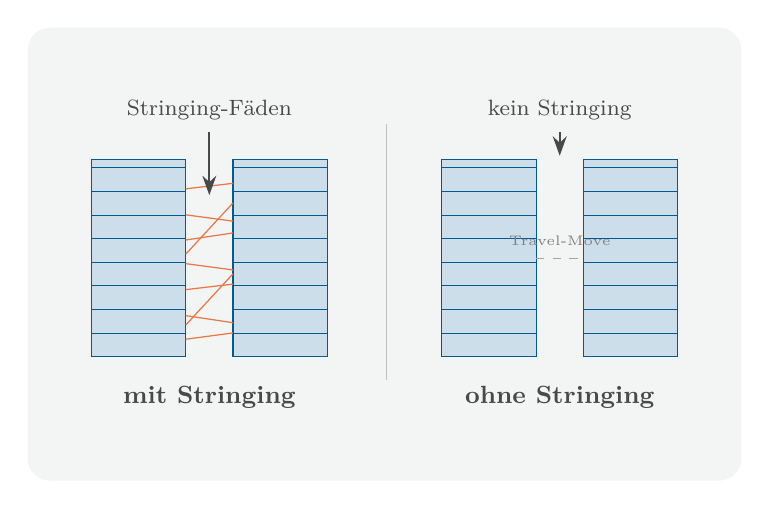
\begin{tikzpicture}[
    show background rectangle,
    background rectangle/.style={fill=my_lightgray, rounded corners=8pt},
    inner frame sep=0.8cm,
    annotation/.style={draw=my_darkgray, thick, -{Stealth[length=7pt, width=5pt]}}
]

%% ================================================================
%% Hilfsmakro: Schichtlinien auf einem Block (sichtbare Layer-Textur)
%% \layerlines{xlinks}{xrechts}{yunten}{yoben}{abstand}
%% ================================================================
\def\blockheight{3.0}
\def\layersep{0.30}

%% ================================================================
%% LINKES PANEL: mit Stringing
%% ================================================================

%% --- Linker Block ---
\fill[fill=my_lightblue, draw=my_darkblue, thin]
    (0.3, 0.5) rectangle (1.5, \blockheight);
\foreach \y in {0.80, 1.10, ..., 3.0} {
    \draw[draw=my_darkblue, very thin] (0.3, \y) -- (1.5, \y);
}

%% --- Rechter Block ---
\fill[fill=my_lightblue, draw=my_darkblue, thin]
    (2.1, 0.5) rectangle (3.3, \blockheight);
\foreach \y in {0.80, 1.10, ..., 3.0} {
    \draw[draw=my_darkblue, very thin] (2.1, \y) -- (3.3, \y);
}

%% --- Stringing-Faeden im Spalt (x: 1.5 bis 2.1) ---
%%     Leicht unregelmaessige Linien fuer realistische Optik
\draw[draw=my_orange, line width=0.45pt] (1.5, 0.72) -- (2.1, 0.80);
\draw[draw=my_orange, line width=0.45pt] (1.5, 1.02) -- (2.1, 0.93);
\draw[draw=my_orange, line width=0.45pt] (1.5, 1.35) -- (2.1, 1.42);
\draw[draw=my_orange, line width=0.45pt] (1.5, 1.68) -- (2.1, 1.60);
\draw[draw=my_orange, line width=0.45pt] (1.5, 1.98) -- (2.1, 2.07);
\draw[draw=my_orange, line width=0.45pt] (1.5, 2.30) -- (2.1, 2.22);
\draw[draw=my_orange, line width=0.45pt] (1.5, 2.63) -- (2.1, 2.70);
%% Diagonale Faeden fuer Unregelmaessigkeit
\draw[draw=my_orange, line width=0.45pt] (1.5, 0.90) -- (2.1, 1.55);
\draw[draw=my_orange, line width=0.45pt] (1.5, 1.80) -- (2.1, 2.45);

%% --- Annotationspfeil: von oben in den Spalt ---
\draw[annotation] (1.80, 3.35) -- (1.80, 2.55);
\node[font=\footnotesize, text=my_darkgray, anchor=south]
    at (1.80, 3.38) {Stringing-Fäden};

%% --- Panel-Label ---
\node[font=\small\bfseries, text=my_darkgray, anchor=north]
    at (1.80, 0.25) {mit Stringing};

%% ================================================================
%% TRENNLINIE zwischen den Panels
%% ================================================================
\draw[draw=my_darkgray!35, thin] (4.05, 0.20) -- (4.05, 3.45);

%% ================================================================
%% RECHTES PANEL: ohne Stringing
%% ================================================================

%% --- Linker Block ---
\fill[fill=my_lightblue, draw=my_darkblue, thin]
    (4.75, 0.5) rectangle (5.95, \blockheight);
\foreach \y in {0.80, 1.10, ..., 3.0} {
    \draw[draw=my_darkblue, very thin] (4.75, \y) -- (5.95, \y);
}

%% --- Rechter Block ---
\fill[fill=my_lightblue, draw=my_darkblue, thin]
    (6.55, 0.5) rectangle (7.75, \blockheight);
\foreach \y in {0.80, 1.10, ..., 3.0} {
    \draw[draw=my_darkblue, very thin] (6.55, \y) -- (7.75, \y);
}

%% --- Sauberer Spalt: gestrichelte Travel-Move-Linie ---
\draw[draw=my_darkgray!50, dashed, thin]
    (5.95, 1.75) -- (6.55, 1.75);
\node[font=\tiny, text=my_darkgray!70, anchor=south]
    at (6.25, 1.78) {Travel-Move};

%% --- Annotationspfeil: sauberer Spalt ---
\draw[annotation] (6.25, 3.35) -- (6.25, 3.05);
\node[font=\footnotesize, text=my_darkgray, anchor=south]
    at (6.25, 3.38) {kein Stringing};

%% --- Panel-Label ---
\node[font=\small\bfseries, text=my_darkgray, anchor=north]
    at (6.25, 0.25) {ohne Stringing};

\end{tikzpicture}

\end{document}
